%%%%%%%%%%%%%%%%%%%%%%%%%%%%%%%%%%%%%%%%%
% Beamer Presentation
% LaTeX Template
% Version 1.0 (10/11/12)
%
% This template has been downloaded from:
% http://www.LaTeXTemplates.com
%
% License:
% CC BY-NC-SA 3.0 (http://creativecommons.org/licenses/by-nc-sa/3.0/)
%
%%%%%%%%%%%%%%%%%%%%%%%%%%%%%%%%%%%%%%%%%

%----------------------------------------------------------------------------------------
%	PACKAGES AND THEMES
%----------------------------------------------------------------------------------------

\documentclass{beamer}

\mode<presentation> {

% The Beamer class comes with a number of default slide themes
% which change the colors and layouts of slides. Below this is a list
% of all the themes, uncomment each in turn to see what they look like.

%\usetheme{default}
%\usetheme{AnnArbor}
%\usetheme{Antibes}
%\usetheme{Bergen}
%\usetheme{Berkeley}
%\usetheme{Berlin}
%\usetheme{Boadilla}
%\usetheme{CambridgeUS}
%\usetheme{Copenhagen}
%\usetheme{Darmstadt}
%\usetheme{Dresden}
%\usetheme{Frankfurt}
%\usetheme{Goettingen}
%\usetheme{Hannover}
%\usetheme{Ilmenau}
%\usetheme{JuanLesPins}
%\usetheme{Luebeck}
\usetheme{Madrid}
%\usetheme{Malmoe}
%\usetheme{Marburg}
%\usetheme{Montpellier}
%\usetheme{PaloAlto}
%\usetheme{Pittsburgh}
%\usetheme{Rochester}
%\usetheme{Singapore}
%\usetheme{Szeged}
%\usetheme{Warsaw}

% As well as themes, the Beamer class has a number of color themes
% for any slide theme. Uncomment each of these in turn to see how it
% changes the colors of your current slide theme.

%\usecolortheme{albatross}
%\usecolortheme{beaver}
%\usecolortheme{beetle}
%\usecolortheme{crane}
%\usecolortheme{dolphin}
%\usecolortheme{dove}
%\usecolortheme{fly}
%\usecolortheme{lily}
%\usecolortheme{orchid}
%\usecolortheme{rose}
%\usecolortheme{seagull}
%\usecolortheme{seahorse}
%\usecolortheme{whale}
%\usecolortheme{wolverine}

%\setbeamertemplate{footline} % To remove the footer line in all slides uncomment this line
%\setbeamertemplate{footline}[page number] % To replace the footer line in all slides with a simple slide count uncomment this line

%\setbeamertemplate{navigation symbols}{} % To remove the navigation symbols from the bottom of all slides uncomment this line
}
\usepackage[T1]{fontenc}

\usepackage{graphicx} % Allows including images
\usepackage{booktabs} % Allows the use of \toprule, \midrule and \bottomrule in tables
\usepackage{array,multirow,graphicx}
\usepackage{todonotes}
\newcommand{\todosk}[1]{\todo[inline]{#1}} 
\usepackage{media9} 

%----------------------------------------------------------------------------------------
%	TITLE PAGE
%----------------------------------------------------------------------------------------

\title[Prova Finale]{Prova Finale} % The short title appears at the bottom of every slide, the full title is only on the title page

\author{Sr\dj{}an Krsti\'c, Claudio Menghi} % Your name
\institute[] % Your institution as it will appear on the bottom of every slide, may be shorthand to save space
{
Politecnico di Milano \\ % Your institution for the title page
\medskip
\textit{srdan.krstic@polimi.it, claudio.menghi@polimi.it} % Your email address
}
\date{\today} % Date, can be changed to a custom date




\begin{document}

\begin{frame}
\titlepage % Print the title page as the first slide
\end{frame}


%----------------------------------------------------------------------------------------
%	PRESENTATION SLIDES
%----------------------------------------------------------------------------------------



\section{Introduzione}
\begin{frame}
\frametitle{Introduzione}
Il progetto consiste nello sviluppo di software del gioco da tavolo.

Il progetto finale dovr\` a includere:
\begin{itemize}
\item diagramma UML iniziale dell'applicazione  (ad alto livello)
\item diagrammi UML finali che mostrino come \`e stato progettato il software;
\item implementazione funzionante del gioco conforme alle regole del gioco e alle specifiche presenti in questo documento
\item codice sorgente dell'implementazione
\item codice sorgente dei test di unit\`a
\end{itemize}
\textbf{La data di consegna: 3 Luglio 2016, AoE}\\
\textbf{La data di valutazione: TBD.}
\end{frame}


{
\usebackgroundtemplate{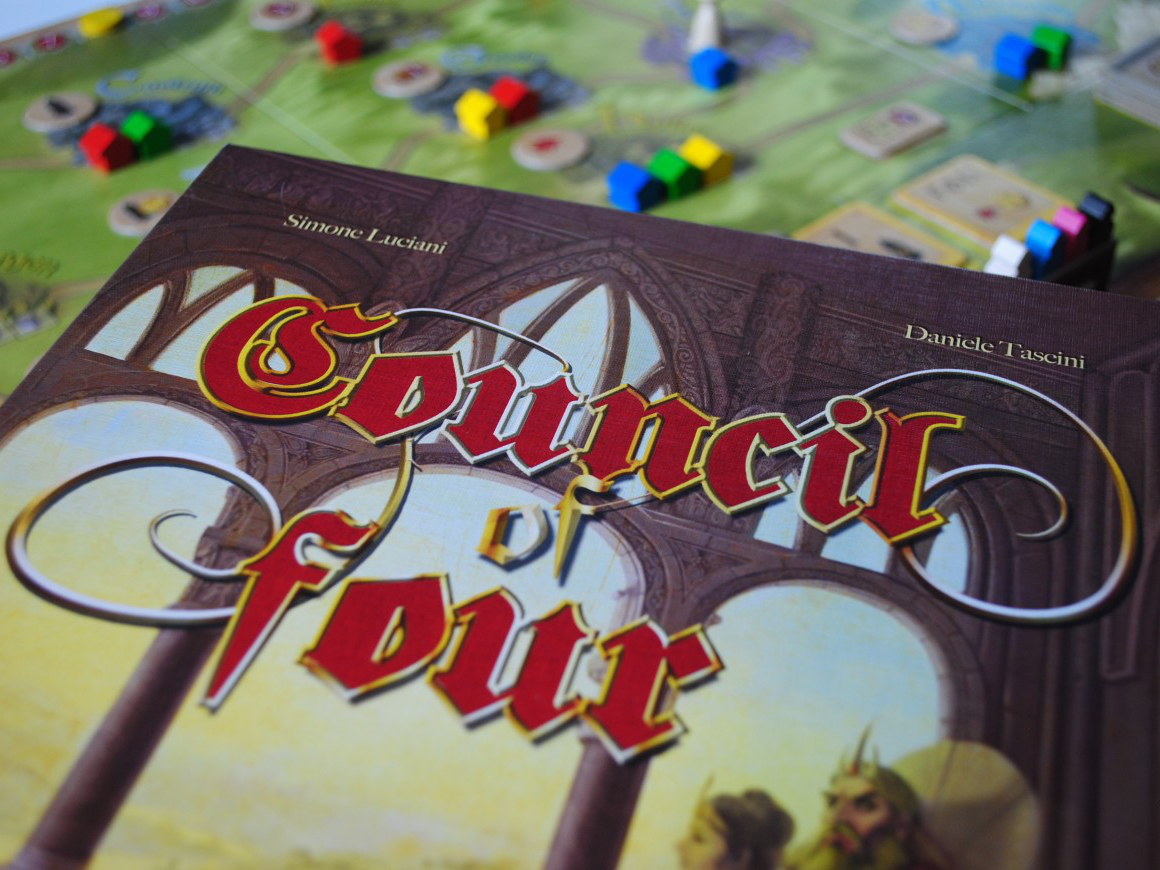
\includegraphics[width=\paperwidth]{cover1.jpg}}%
\section{Council of Four (CoF)}
\begin{frame}[plain]


\end{frame}
}

\section{Requirements}

\subsection{Regole}

\begin{frame}

\LARGE	
\textbf{Game-specific requirements}

\end{frame}

\begin{frame}
  \frametitle{Regole base}

\begin{itemize}
\item Regole ufficiale del gioco sono descritte nel file \textbf{GameRules.pdf}
(Inglese) e \textbf{RegoleGioco.pdf} (Italiano), caricati su BeeP.

\item Ci sono buone spiegazioni anche su Youtube:

{\footnotesize
  \url{https://www.youtube.com/v/8fhU9SiI4eE?start=87&end=491&vq=hd1080}
}
\end{itemize}
\end{frame}

\begin{frame}
  \frametitle{Regole Addizionali}

\begin{itemize}
\item \textbf{Gioco configurabile}: 
il gioco deve essere progettato al fine di poter creare:
\begin{enumerate}
\item mappa configurabile
\begin{enumerate}
\item connessioni arbitrarie tra le citt\'a;
\item bonus arbitrari;
\item numero di bonus arbitrari;
\end{enumerate}
\item numero arbitrario di giocatori;
\item file di configurazione con lista di mappe (con 3 punti
  sopra). Numero dei giocatori deve essere un parametro alla creazione
  del gioco;
\end{enumerate}
\item \textbf{Market}: dopo che tutti i giocatori hanno giocato il
  loro turno (dopo ogni giro) viene lanciata la fase di Market.
 Partendo dal primo giocatore  fino all'ultimo, ogni giocatore pu\' o
 scegliere le carte (di permesso e politiche) e gli assistenti che intende vendere e il
 prezzo richiesto per ognuno di essi.
 Quando TUTTI i giocatori hanno scelto quali elementi vendere,
seguendo un ordine casuale i giocatori possono comprare gli elementi messi in vendita dagli altri giocatori.


\end{itemize}
\end{frame}


\subsection{Specifiche implementative}

\begin{frame}
\LARGE	
\textbf{Game-agnostic requirements}

\end{frame}

\begin{frame}
\frametitle{Specifiche implementative}
In questa sezione vengono presentati i requisiti tecnici
dell'applicazione.  Deve essere un sistema distributivo composto da
un lato gioco che pu\'o gestire molti giochi simultanei e multipli
lati giocatore che possono partecipare nel un solo gioco. Si raccomanda
l'utilizzo del pattern \textbf{MVC} (Model-View-Controller) per
progettare l'intero sistema.
\end{frame}

\subsubsection{Lato Giocatore}
\begin{frame}
\frametitle{Lato Giocatore}
\begin{itemize}
\item Il lato giocatore deve poter essere istanziato pi\`u volte. 
\item Il lato giocatore deve essere sviluppato obbligatoriamente utilizzando JavaSE. 
\item L'interfaccia grafica deve essere mediante Swing o altre
  tecnologie (tuttavia in questo caso non sarete supportati dai responsabili), 
\item Il lato giocatore deve supportare RMI e Socket, in relazione al numero di studenti del gruppo, come specificato in tabella~\ref{TabellaDiValutazione}. 
\item Nel caso in cui sia richiesta sia l'implementazione RMI che
  quelle per mezzo di socket, l'applicazione, all'avvio, deve permettere
  all'utente di selezionare il metodo utilizzato per la
  comunicazione.
\item Nel caso in cui sia richiesta sia l'implementazione CLI che
  quelle per mezzo di GUI, l'applicazione, all'avvio, deve permettere
  all'utente di selezionare il metodo utilizzato per la
  visualizzazione.
\end{itemize}
\end{frame}

\subsubsection{Lato Gioco}
\begin{frame}
\frametitle{Lato Gioco}
Questo componente deve gestire le partite e deve poter essere
istanziato una sola volta. Deve permettere di:
\begin{itemize}
\item creare una nuova partita, inizializzarla, giocarla e concluderla secondo le regole del gioco.
\item Deve essere in grado di gestire pi\`u partite
  contemporaneamente.
\item Deve essere implementato secondo la logica JavaSE.
\item Nel caso in cui sia l'implementazione via socket che quelle via
  RMI sia richiesta, quando un giocatore si connette al server, il server deve comunicare utilizzando la connessione selezionata.
\end{itemize}
\end{frame}

\subsubsection{Avvio della partita}
\begin{frame}
\frametitle{Avvio della partita}
L'assunzione base \`e che ogni giocatore che voglia partecipare a
una partita conosca l'indirizzo (numerico o simbolico) del lato gioco. Quando un giocatore si connette, 
\begin{itemize}
\item se c\`e una partita in fase di avvio, il giocatore viene automaticamente aggiunto alla partita
\item  \textbf{Regole base:\footnote{se non sono richeste le regole
      addizionali}} la partita inizia non appena si raggiungono i 4
  giocatori. Quando 2 giocatori si connettono a una partita viene
  inizializzato un timeout di 20 secondi. Non appena il timeout scatta
  la partita inizia anche se non sono raggiunti i 4 giocatori.
\item  \textbf{Regole complete:\footnote{se sono richeste le regole
      addizionali}} quando 2 giocatori si connettono a una partita viene
  inizializzato un timeout di 20 secondi. Non appena il timeout scatta
  la partita inizia. Il numero di giocatori pu\'o essere arbitrario,
  anche maggiore di 4.
\item se non ci sono partite in fase di avvio, viene creata una nuova partita.
\end{itemize}
Si precisa che una nuova partita viene creata solamente quando un utente si connette e non ci sono partite in attesa, altrimenti l'utente entra automaticamente a far parte della partita in fase di avvio.
\end{frame}

\subsubsection{Corso della partita}
\begin{frame}
\frametitle{Corso della partita}
Il lato gioco consente ai vari giocatori di svolgere i propri turni
secondo le regole di gioco. E' necessario gestire il caso in cui i
lati giocatore si disconnettano.
\begin{itemize}
\item ogni giocatore ha un periodo di tempo fissato passato come parametro al momento della creazione del server per  eseguire le mosse 
\item se un giocatore va offline il lato gioco attende per il periodo di
  cui sopra,
  dopo il quale sospende il giocatore (nota il giocatore non esegue
  mosse ma viene comunque considerato nel conteggio dei punti etc.) 
\item tutti i giocatori vengono notificati della mancanza di un giocatore
\item il gioco continua, saltando i giri del giocatore sospeso
\item il lato giocatore pu\'o riconnettersi e continuare il gioco se si
  sceglie di implementare la funzionalit\'a ``Ripristino sessione giocatore''.
\end{itemize}
\end{frame}

\section{Funzionalita Avanzate}
\begin{frame}
\LARGE	
\textbf{Funzionalita Avanzate}

\end{frame}

\begin{frame}
\frametitle{Funzionalita Avanzate}

Di seguito sono proposte alcune funzionalit\`a avanzate che concorrono alla valutazione.  Attenzione: il loro contributo non \`e  necessariamente additivo. Design e codice verranno comunque valutati in quanto tali e contribuiranno al giudizio globale.

\begin{itemize}
\item \textbf{Gestione degli utenti}
\item  \textbf{Lato Gioco persistente}
\item  \textbf{Ripristino sessione giocatore}
\item \textbf{Generazione automatica delle configurazioni di gioco}
\item \textbf{Lobby}
\item \textbf{Chat}
\item \textbf{AI}

%TODO: this requirements are underspecified on purpose, so that you
%can creatively contribute to your own project the way you want

\end{itemize}
\end{frame}


\section{Valutazione}

\begin{frame}
\LARGE	
\textbf{Valutazione}

\end{frame}

\begin{frame}
\frametitle{Valutazione}
Saranno oggetto di valutazione
\begin{itemize}
\item la qualit\` a della \textbf{progettazione} con particolare riferimento a
  un uso appropriato di interfacce, ereditariet\`a, composizione tra
  classi, uso dei design pattern;
\item la qualit\` a della progettazione dell'\textbf{architettura
  dell'applicazione}; divisione della responsabilit\'a; progettazione
  della comunicazione;
\item la stabilit\` a dell'implementazione e la \textbf{conformit\` a alle
  specifiche} date; 
\item la \textbf{qualit\` a} e la \textbf{leggibilit\` a} del codice scritto, con
  particolare riferimento a nomi di variabili/metodi/classi/package,
  all'inserimento di commenti e documentazione JavaDoc
  (preferibilmente in inglese), la mancanza di codice ripetuto e
  metodi di eccessiva lunghezza;
\item la \textbf{qualit\` a} e la \textbf{copertura} dei casi di test: il nome e i
  commenti di ogni test dovranno chiaramente specificare le funzionalit\`
  a testate e i componenti coinvolti;
 \item il corretto utilizzo degli strumenti (Eclipse, Git, Maven, ...);
\item il livello di autonomia e impegno nello svolgimento del progetto.
\end{itemize}
\end{frame}



\begin{frame}
\frametitle{Valutazione - Acronimi}
\begin{itemize}
\item \textbf{Command Line Interface (CLI)}: \`e implementato come un'interfaccia testuale e i vari giocatori si alternano nei turni utilizzando la tastiera.
\item \textbf{GUI}: consiste in un interfaccia grafica swing
\item \textbf{RMI:} la comunicazione avviene mediante ``Remote method invocation''
\item \textbf{Socket}: la comunicazione avviene mediante messaggi scambiati
  attraverso socket. Lo studente deve autonomamente definire e
  implementare un protocollo di comunicazione tra i componenti distribuiti.
\end{itemize}
\end{frame}



\begin{frame}
\frametitle{Valutazione}
\small

\begin{table}[b]
  \centering
\newcolumntype{B}{>{\raggedright\arraybackslash}m{0.5cm}}

\begin{tabular}{ B c c c  }
\toprule
\setlength{\columnsep}{0.01cm}

Voto & \multicolumn{3}{c}{Numero studenti} \\

Max & 1 & 2 & 3 \\

\midrule 
18 &
Regole base&
Regole complete & 
Regole complete \\

22 &
CLI + GUI &
RMI + CLI & 
Socket + CLI \\

24 & 
RMI + CLI &
Socket + CLI  &
RMI + Socket + CLI \\

26 &
Socket + CLI &
RMI + Socket + CLI &
RMI + Socket + GUI\\

28 &
RMI + Socket + CLI &
RMI + Socket + GUI &
All Tech\\

30L &
RMI + Socket + GUI &
All Tech &   
1 Funzionalit\`a Avanzata\\

\bottomrule
\end{tabular}
\caption{Tabella di valutazione}
\label{TabellaDiValutazione}
\end{table}


La tabella di valutazione presenta le funzionalit\`a da implementare
nel caso di gruppi da 2 e 3 studenti.
Gli studenti di telecomunicazioni, possono fare i gruppi insieme di un
massimo di 4 persone ed i requisiti applicati corrisponderanno al
gruppo con una persona in meno, con l'eccezione di un gruppo di 1
persona. 
\textbf{Non \`e possibile fare i gruppi di 1 persona, la
  tabella~\ref{TabellaDiValutazione} contiene le informazioni solo
  come riferimento agli studenti di telecomunicazioni.}

\end{frame}



\begin{frame}
\frametitle{Valutazione}
I gruppi da 2 o 3 studenti devono implementare  le specifiche
descritte in tabella~\ref{TabellaDiValutazione} in relazione al
punteggio desiderato. Nota: in tabella sono rappresentati i
\textbf{massimi} punteggi ottenibili in relazione alle features
implementate. Per esempio, per un gruppo di 2 studenti e un punteggio
desiderato di al massimo 24 punti \`e necessario implementare:
comunicazione con Socket e il Command Line Interface (CLI).
All Tech significa che il gruppo deve implementare i due modi di
comunicazione (RMI e Socket) e i due tipi di Interface (CLI e GUI).

Le funzionalit\`a avanzate possono essere implementate da tutti gruppi e comportano punteggi aggiuntivi. Ovviamente per implementare queste funzionalit\`a \`e necessario che TUTTO il resto del progetto sia implementato in maniera COMPLETA e ADEGUATA (copertura con test, ben commentata etc).
\end{frame}



{
\usebackgroundtemplate{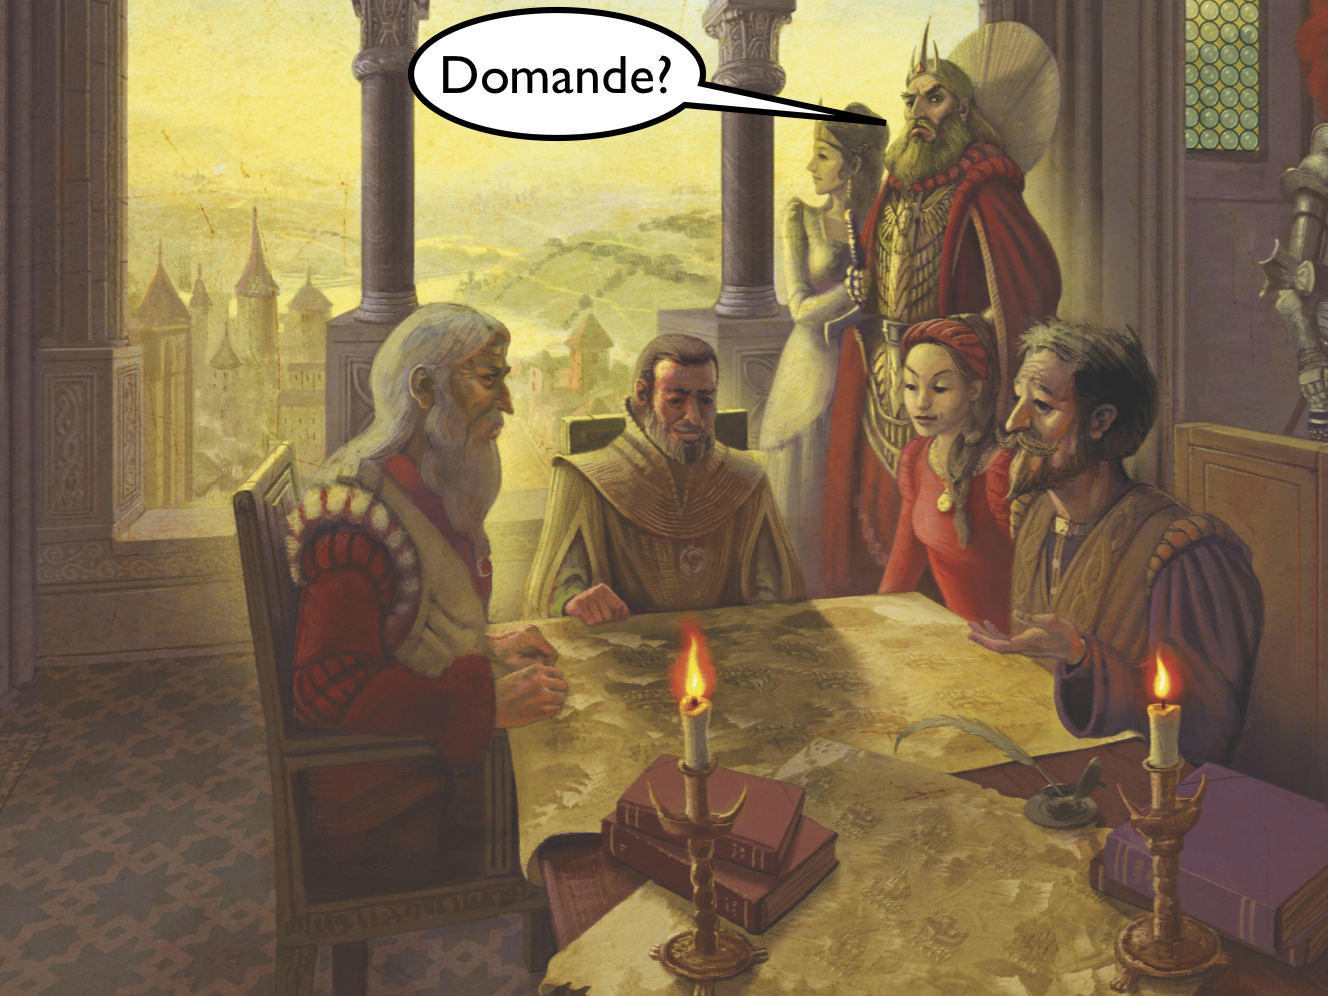
\includegraphics[width=\paperwidth]{domande.jpg}}%
\section{Council of Four}
\begin{frame}[plain]



\end{frame}
}



\subsection{Organizzazione Laboratorio}
\begin{frame}
\frametitle{Organizzazione Laboratorio}


\begin{table}
  \centering
\footnotesize

\begin{tabular}{ l l l }
\toprule

\setlength{\columnsep}{0.01cm}

Date & Format & Topics \\
\midrule
  12 Aprile & P & \textbf{Focus:} Groups, Eclipse, Maven, Git, Sonar\\
  && \textbf{Checkpoint:} Installed Eclipse, Formed groups \& repositories\\
  19 Aprile & D & \textbf{Focus:} UML design (Model), Architexa \\
  && \textbf{Checkpoint:} Created project, Maven, Git, Sonar \\
  10 Maggio & D & \textbf{Focus:} Architecture design (MVC) \\
  && \textbf{Checkpoint:} UML design (Model) \\
  24 Maggio & P/D & \textbf{Focus:} Testing, JUnit, TDD \\
  && \textbf{Checkpoint:} Architecture design (MVC), Implementation\\
  31 Maggio & P/D & \textbf{Focus:} Communication, Multithreading and Protocol design\\
  && \textbf{Checkpoint:} Test coverage and documentation\\
  7 Giugno & D & \textbf{Focus:} General Discussion \\
  && \textbf{Checkpoint:} Communication implementation\\
  14 Giugno & P/D & \textbf{Focus:} Swing and GUI design \\
  && \textbf{Checkpoint:} Implementation\\
  21 Giugno & D & \textbf{Focus:} General Discussion and Deployment \\
  && \textbf{Checkpoint:} GUI design and Implementation\\

\bottomrule
\end{tabular}
\caption{Lab schedule (P = Presentation, D = Discussion)}
\label{schedule}
\end{table}

\end{frame}

\subsection{TODO}
\begin{frame}
\frametitle{TODO (entro 12/04/2016)}
\begin{enumerate}
\item Create un'account su BitBucket (\url{https://bitbucket.org/})
\item Formate i gruppi
\item Un membro del gruppo deve creare un repository in BitBucket,
  aggungere i propri compagni come ``admin'' o ``write''
\item E aggungere nostro account con username "krle" (Srdjan Krstic)
  come ``read''.
\item Completate il modulo (una persona per gruppo): 
\url{http://goo.gl/forms/UIutpuCoaa}
\item Installate gli strumenti (riferimento a ``beep'' per le guide su
  Eclipse, Sonar e Architexa)
\item Leggete le regole del gioco e le requisiti di progetto
  (riferimento a "beep"). Preparate domande. Iniziate le discussioni su BEEP.

\end{enumerate}
\end{frame}



\end{document} 

